\documentclass[floatsintext,man]{apa6}

\usepackage{amssymb,amsmath}
\usepackage{ifxetex,ifluatex}
\usepackage{fixltx2e} % provides \textsubscript
\ifnum 0\ifxetex 1\fi\ifluatex 1\fi=0 % if pdftex
  \usepackage[T1]{fontenc}
  \usepackage[utf8]{inputenc}
\else % if luatex or xelatex
  \ifxetex
    \usepackage{mathspec}
    \usepackage{xltxtra,xunicode}
  \else
    \usepackage{fontspec}
  \fi
  \defaultfontfeatures{Mapping=tex-text,Scale=MatchLowercase}
  \newcommand{\euro}{€}
\fi
% use upquote if available, for straight quotes in verbatim environments
\IfFileExists{upquote.sty}{\usepackage{upquote}}{}
% use microtype if available
\IfFileExists{microtype.sty}{\usepackage{microtype}}{}

% Table formatting
\usepackage{longtable, booktabs}
\usepackage{lscape}
% \usepackage[counterclockwise]{rotating}   % Landscape page setup for large tables
\usepackage{multirow}		% Table styling
\usepackage{tabularx}		% Control Column width
\usepackage[flushleft]{threeparttable}	% Allows for three part tables with a specified notes section
\usepackage{threeparttablex}            % Lets threeparttable work with longtable

% Create new environments so endfloat can handle them
% \newenvironment{ltable}
%   {\begin{landscape}\begin{center}\begin{threeparttable}}
%   {\end{threeparttable}\end{center}\end{landscape}}

\newenvironment{lltable}
  {\begin{landscape}\begin{center}\begin{ThreePartTable}}
  {\end{ThreePartTable}\end{center}\end{landscape}}




% The following enables adjusting longtable caption width to table width
% Solution found at http://golatex.de/longtable-mit-caption-so-breit-wie-die-tabelle-t15767.html
\makeatletter
\newcommand\LastLTentrywidth{1em}
\newlength\longtablewidth
\setlength{\longtablewidth}{1in}
\newcommand\getlongtablewidth{%
 \begingroup
  \ifcsname LT@\roman{LT@tables}\endcsname
  \global\longtablewidth=0pt
  \renewcommand\LT@entry[2]{\global\advance\longtablewidth by ##2\relax\gdef\LastLTentrywidth{##2}}%
  \@nameuse{LT@\roman{LT@tables}}%
  \fi
\endgroup}


  \usepackage{graphicx}
  \makeatletter
  \def\maxwidth{\ifdim\Gin@nat@width>\linewidth\linewidth\else\Gin@nat@width\fi}
  \def\maxheight{\ifdim\Gin@nat@height>\textheight\textheight\else\Gin@nat@height\fi}
  \makeatother
  % Scale images if necessary, so that they will not overflow the page
  % margins by default, and it is still possible to overwrite the defaults
  % using explicit options in \includegraphics[width, height, ...]{}
  \setkeys{Gin}{width=\maxwidth,height=\maxheight,keepaspectratio}
\ifxetex
  \usepackage[setpagesize=false, % page size defined by xetex
              unicode=false, % unicode breaks when used with xetex
              xetex]{hyperref}
\else
  \usepackage[unicode=true]{hyperref}
\fi
\hypersetup{breaklinks=true,
            pdfauthor={},
            pdftitle={Final Project},
            colorlinks=true,
            citecolor=blue,
            urlcolor=blue,
            linkcolor=black,
            pdfborder={0 0 0}}
\urlstyle{same}  % don't use monospace font for urls

\setlength{\parindent}{0pt}
%\setlength{\parskip}{0pt plus 0pt minus 0pt}

\setlength{\emergencystretch}{3em}  % prevent overfull lines


% Manuscript styling
\captionsetup{font=singlespacing,justification=justified}
\usepackage{csquotes}
\usepackage{upgreek}

 % Line numbering
  \usepackage{lineno}
  \linenumbers


\usepackage{tikz} % Variable definition to generate author note

% fix for \tightlist problem in pandoc 1.14
\providecommand{\tightlist}{%
  \setlength{\itemsep}{0pt}\setlength{\parskip}{0pt}}

% Essential manuscript parts
  \title{Final Project}

  \shorttitle{Final Project}


  \author{Nate Koser}

  % \def\affdep{{""}}%
  % \def\affcity{{""}}%

  \affiliation{
    \vspace{0.5cm}
          \textsuperscript{} Rutgers University  }



  \keywords{keywords \\

    \indent Word count: X
  }





\usepackage{amsthm}
\newtheorem{theorem}{Theorem}
\newtheorem{lemma}{Lemma}
\theoremstyle{definition}
\newtheorem{definition}{Definition}
\newtheorem{corollary}{Corollary}
\newtheorem{proposition}{Proposition}
\theoremstyle{definition}
\newtheorem{example}{Example}
\theoremstyle{definition}
\newtheorem{exercise}{Exercise}
\theoremstyle{remark}
\newtheorem*{remark}{Remark}
\newtheorem*{solution}{Solution}
\begin{document}

\maketitle

\setcounter{secnumdepth}{0}



\subsection{Introduction}\label{introduction}

This paper is an investigation of drunk driving patterns in South Korea
for the year 2016. The data were obtained from
\href{http://kosis.kr/index/index.do}{kosis.kr}, the Korean Statistical
Information Service website maintained by the National Statistical
Office. The data include information on the number of cases, deaths, and
injuries resulting from drunk driving incidents organized by time of
day, month of the year, and level of intoxication.

\subsection{Hypotheses}\label{hypotheses}

The analysis presented here is an investigation of three main
hypotheses. The first is that the number of cases that occured will be a
good predictor for time of day (day or night), and that generally there
are more incidents at night. The second is that there will be more cases
in months with major holidays. These months will include
December/January - when solar new year's day occurs; February - when
lunar new year's day occurs; and September - when the fall harvest
holiday (similar to Thanksgiving in North America) occurs. The third
hypothesis to be tested involves high levels of intoxication. Within the
\texttt{abv} variable, there is a value \enquote{\textgreater{}.35\%},
indicating a blood alcohol content of over .35\%. The hypothesis is that
at this extreme level of intoxication, the risk of death will be
greater. Descriptive statistics, plots, and model information for all
three hypotheses will be provided in the following sections.

\subsection{Data analysis}\label{data-analysis}

\emph{Day and Night}

The following table shows a summary of some descriptive statistics
regarding the general occurance of drunk driving during the night and
during the day. The numbers given are log-adjusted.

\begin{longtable}[]{@{}lrrrr@{}}
\toprule
timeofday & CasesMean & CasesSd & InjuriesMean &
InjuriesSd\tabularnewline
\midrule
\endhead
day & 2.92 & 1.63 & 3.40 & 1.73\tabularnewline
night & 3.58 & 2.01 & 4.05 & 2.09\tabularnewline
\bottomrule
\end{longtable}

We observe a higher mean incidence of cases during the night than during
the day, as well as a higher mean number of injuries during the night
vs.~the day. This is line with our proposed hypothesis.

The following is a plot of a binomial regression where a value of 1
indicates \enquote{day} and a value of 0 indicates \enquote{night}. The
predictor is the number of cases that occured.

\begin{figure}
\centering
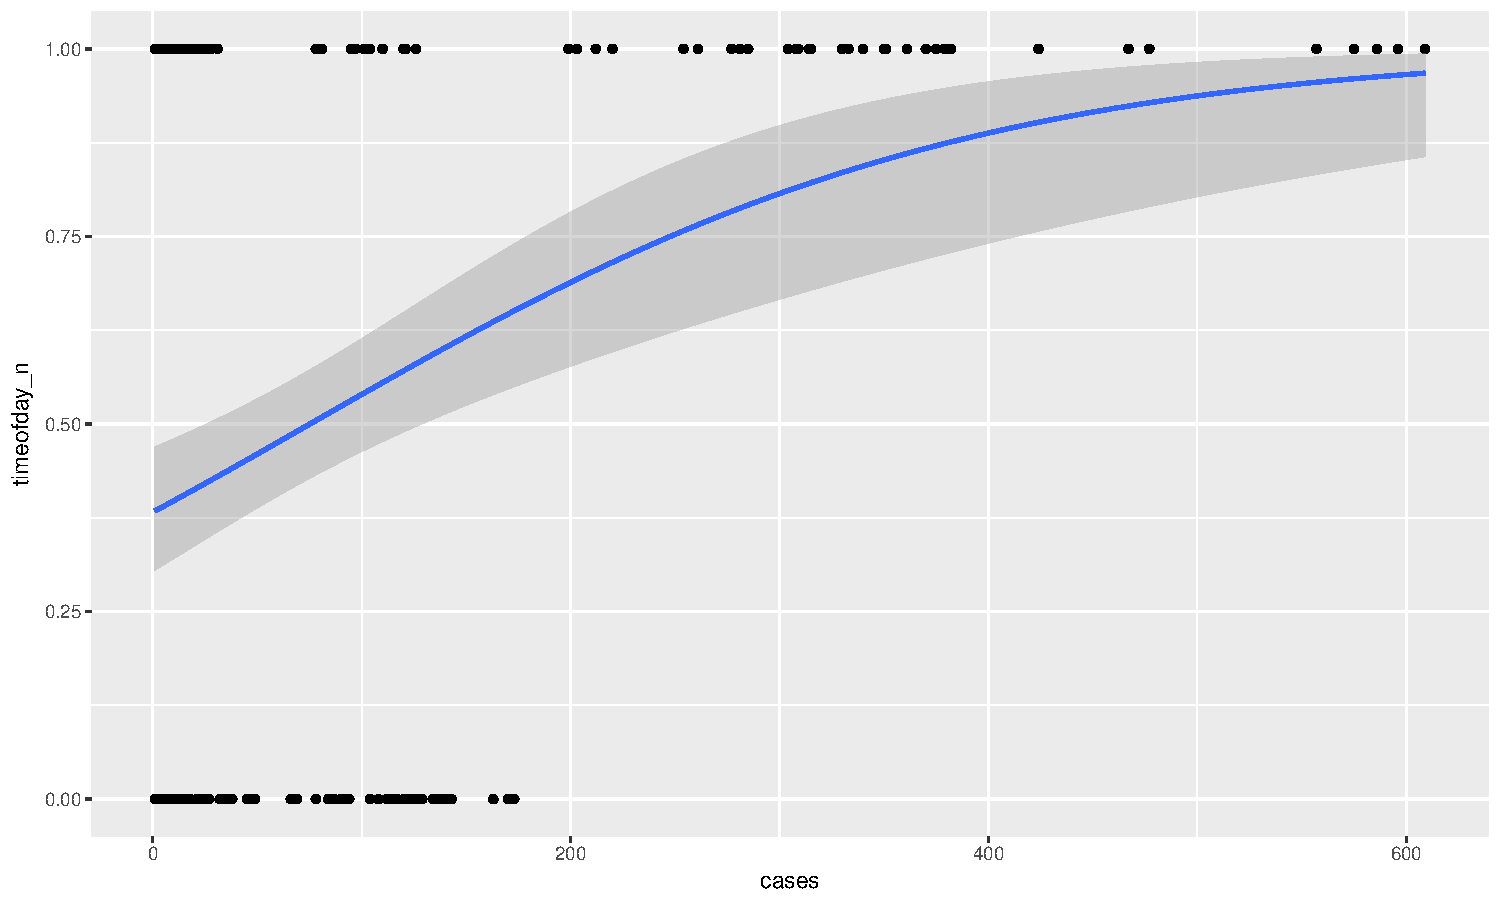
\includegraphics{final_files/figure-latex/daynight-1.pdf}
\caption{}
\end{figure}

Visual inspection reveals a general upward trend towards nighttime as
the number of cases increases. In fact, the max number of cases occuring
in any one daytime period (\textasciitilde{}180) appears to be much
lower than the max number of cases occuring on the busiest night
(\textgreater{}600). The shape of the curve reflects this and it is once
again amenable to the stated hypothesis.

A generalized linear model was fit to the data using a binomial
regression with a logit linking function. The following table is a
summary of the results of this model fit.

\begin{longtable}[]{@{}lllll@{}}
\toprule
term & estimate & std. error & z value & p value\tabularnewline
\midrule
\endhead
(Intercept) & -0.48 & 0.18 & -2.66 & \textless{} 0.01 *\tabularnewline
cases & 0.01 & 0.001 & 4.25 & \textless{} 0.001 **\tabularnewline
\bottomrule
\end{longtable}

We see that there is a significant effect of cases as a predictor for
night or day in the data (\emph{p}-value \textless{}0.001). Taking the
inverse logit of the estimates for the night-day intercept and cases
reveals a 62\% chance of the incident having occured at night when the
number of cases equals 100, and an increase in this chance by
\textasciitilde{}20\% when the number of cases is 200. Increasing the
number of cases to 300 reflects a further \textasciitilde{}10\% increase
in the probability of the event occuring at night, up to 92.55\%. These
results are reflective of the trend observed in the plot above.

\emph{Months of the Year}

The following table shows a summary of some descriptive statistics
regarding the general occurance of drunk driving during different months
of the year. The numbers given are log-adjusted.

\begin{longtable}[]{@{}lrrrr@{}}
\toprule
month & CasesMean & CasesSd & InjuriesMean & InjuriesSd\tabularnewline
\midrule
\endhead
April & 3.43 & 1.93 & 4.00 & 1.83\tabularnewline
August & 3.26 & 1.86 & 3.68 & 2.02\tabularnewline
December & 3.30 & 2.05 & 3.68 & 2.25\tabularnewline
February & 3.16 & 1.99 & 3.78 & 1.90\tabularnewline
January & 3.22 & 1.93 & 3.61 & 2.13\tabularnewline
July & 3.06 & 2.01 & 3.55 & 2.02\tabularnewline
June & 3.10 & 1.80 & 3.55 & 1.95\tabularnewline
March & 3.31 & 1.94 & 3.82 & 1.96\tabularnewline
May & 3.38 & 1.80 & 3.93 & 1.79\tabularnewline
November & 3.36 & 2.01 & 3.74 & 2.20\tabularnewline
October & 3.34 & 1.87 & 3.81 & 2.00\tabularnewline
September & 3.25 & 1.75 & 3.74 & 1.88\tabularnewline
\bottomrule
\end{longtable}

The months described in the hypothesis above do not appear to have any
special status in terms of the number of cases or injuries that occur.
In particular, Janurary and February's cases and inuries are among the
lowest, while April sticks out as being the most active. Also of note is
the standard deviation values, which are more than 50\% of the
corresponding mean for most values in the table. This indicates data
that is more spread out, and less concentrated around any one point (the
mean).

\emph{Figure 2} is a boxplot of the log cases of drunk driving with the
month as the predictor.

\begin{figure}
\centering
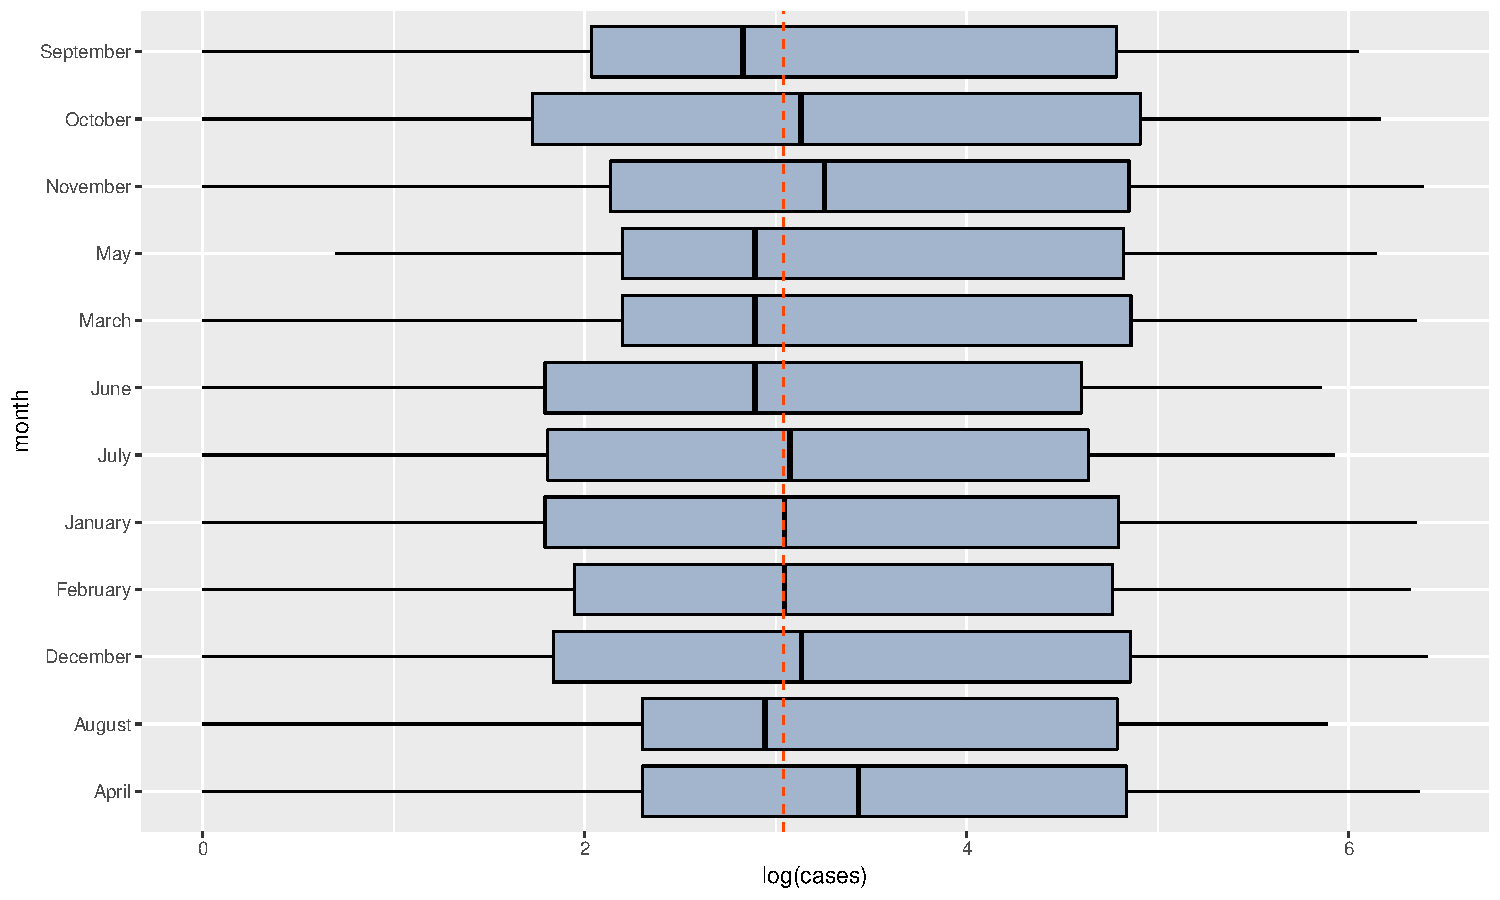
\includegraphics{final_files/figure-latex/bymonth-1.pdf}
\caption{}
\end{figure}

The median of the log cases for all months is 3.04, and the vertical red
line in the plot marks this value. Visual inspection reveals that the
median of the log case value for January and February is right on the
the red line. The value for December is slightly above it, and the value
for September appears to be lower. This is not in line with the proposed
hypothesis. Unexpectedly, April shows the biggest departure from the
median value - it is the highest above the red line.

As December is the month among our hypothesized months with the highest
mean and median cases, it makes sense to isolate it as a \enquote{best
case scenario} and fit models considering it. To this end, I fit a
binomial generalized linear model to the data, where a response of 1
indicates that the event occured in December, and a response of 0
indicates that the even occured in some other month. The results are
summarized in the table below.

\begin{longtable}[]{@{}lllll@{}}
\toprule
term & estimate & std. error & z value & p value\tabularnewline
\midrule
\endhead
(Intercept) & -2.56 & 0.32 & -7.95 & \textless{} 0.001**\tabularnewline
cases & 0.001 & 0.002 & 0.5 & 0.6\tabularnewline
\bottomrule
\end{longtable}

No significant effect of cases was found on an event occuring in
December or not. An investigation of inverse logit values reveals an 8\%
chance of having occured in December when the number of cases is equal
to 100. An increase to 200 cases comes with a positive change of
\textless{}1\% probability of being in December, and a further increase
to 300 cases has the same result, raising the probability to only 9.4\%.
None of the methods employed here confirm our hypothesis that drunk
driving incidents are more frequent in months with a major holiday.

\emph{High Blood Alcohol Content}

The following table shows a summary of some descriptive statistics
regarding drunk driving at a measured blood alcohol content of over and
under .35\% and the mean deaths per case for each category. The numbers
given are log-adjusted.

\begin{longtable}[]{@{}ll@{}}
\toprule
BAC & Deaths as percent of cases\tabularnewline
\midrule
\endhead
over .35 & 0.03\tabularnewline
under .35 & 0.02\tabularnewline
\bottomrule
\end{longtable}

The numbers indicate that there is a slightly higher chance of death at
the advanced BAC of \textgreater{}.35\% than there is for lower BAC
values.

The following is the plot of a binomial regression where a response of 1
indicates that the event occured at a BAC of \textgreater{}.35\%, and a
response of 0 indicates otherwise.

\begin{figure}
\centering
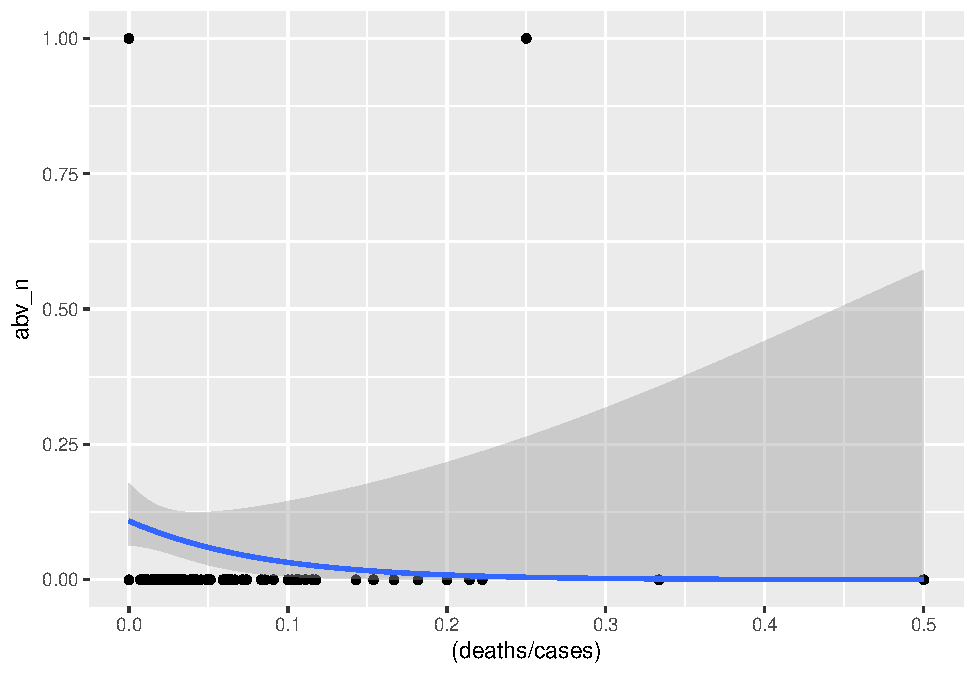
\includegraphics{final_files/figure-latex/deathplot-1.pdf}
\caption{}
\end{figure}

The plot indicates that there is a slight negative trend - as the number
of deaths per cases increases, the chance that the incident in question
occured at a BAC value of \textgreater{}.35\% decreases. This is not
what the descriptive statistics in the table above indicated. This may
be due to the scarcity of cases occuring at such a high BAC - the larger
number of cases where a larger propotion of people died at a lower BAC
could offset the fewer number of cases at a higher BAC.

The following table is the result of fitting a generalized linear model
with a binomial, logit linking function to the data.

\begin{longtable}[]{@{}lllll@{}}
\toprule
term & estimate & std. error & z value & p value\tabularnewline
\midrule
\endhead
(Intercept) & -2.11 & 0.29 & -7.21 & \textless{} 0.001**\tabularnewline
deathchance & -13.04 & 9.37 & -1.39 & 0.16\tabularnewline
\bottomrule
\end{longtable}

There is what could be considered a non-significant trend (p = .16) for
chance of death when being invovled in an incident at a BAC of over
.35\%. This trend is negative, as can be observed in the plot. Taking
the inverse logit indicates a 10.8\% chance of the incident occuring at
a BAC of over .35\% when the number of deaths per case is equal to zero.
When the deaths per case increases to .5, the chance of having occured
at BAC \textgreater{}.35\% is a mere .02\%. This does not confirm the
hypothesis that more deaths occur at a higher blood alcohol content.

\subsection{Discussion}\label{discussion}

In the preceding analysis, three hypotheses were proposed and analyzed.
The first hypothesis was that there are more cases of drunk driving
during the night than during the day. Statistical analysis through
generalized linear models revealed that this is the case - there was a
significant effect of number of cases on time of occurance
(\emph{p}-value \textless{} 0.001).

The second hypothesis was that more drunk driving incidents occur in
months that have major holidays. These included September, December,
January, and February. Statistical anaylsis showed that there is no such
effect. For the month of December, which was determined ot be the most
hopeful in terms of the hypothesis, there was only a slight positive
trend which was not found to be statistically significant
(\emph{p}-value \textless{} 0.6).

The third hypothesis was that at the high BAC level of
\textgreater{}.35\%, there would be a higher number of deaths per
incident of drunk driving. While examination of the mean initially
suggested that this may be the case, there was no statistically
significant effect found in support of the hypothesis. In fact, a
general negative trend was found (\emph{p}-value .16). This
non-intuitive result may be due to the dearth of cases at this high BAC
- visual inspection of the data set reveals that they are only a tiny
portion of the overall number of cases. It is possible that
incorporation of more data would reverse this trend.

\begin{center}\rule{0.5\linewidth}{\linethickness}\end{center}

\setlength{\parindent}{-0.5in} \setlength{\leftskip}{0.5in}






\end{document}
